\documentclass[11pt]{article}

\usepackage[margin=1in]{geometry}
\usepackage{setspace}
\onehalfspacing
\usepackage{graphicx}
\graphicspath{report_images/}
\usepackage{appendix}
\usepackage{listings}
\usepackage{float}
\usepackage{multirow}
\usepackage{amsthm}
% The next three lines make the table and figure numbers also include section number
\usepackage{chngcntr}
\counterwithin{table}{section}
\counterwithin{figure}{section}
% Needed to make titling page without a page number
\usepackage{titling}
% Needed to use cent symbol
\usepackage{textcomp}
% Needed to use greater than or equal to
\usepackage{amssymb}

% DOCUMENT INFORMATION =================================================
\font\titleFont=cmr12 at 11pt
\title {{\titleFont ECEN 429: Introduction to Digital Systems Design Laboratory \\ North Carolina Agricultural and Technical State University \\ Department of Electrical and Computer Engineering}} % Declare Title
\author{\titleFont Reporter: Chris Cannon \\ Partner: Nikiyah Beulah} % Declare authors
\date{\titleFont April 12, 2018}
% ======================================================================

\begin{document}

\begin{titlingpage}
\maketitle
\begin{center}
	Prelab 10
\end{center}
\end{titlingpage}

\section{Introduction}
The purpose of this prelab is to evaluate the state machine involved in a Vending Machine, and to utilize state minimization.

\section{Background, Design Solution, Results}

\subsection{Problem 2}
For Step 2: what does each state mean (e.g. what does it mean if the FSM is in State S0, S1, etc)?

\begin{table}[H]
\begin{center}
\begin{tabular}{| l | l |}
	\hline
	State & Meaning \\ \hline
	S0 & Nothing Deposited \\ \hline
	S1 & 1 Nickel \\ \hline
	S2 & 1 Dime \\ \hline
	S3 & 2 Nickels \\ \hline
	S4 & 1 Nickel, 1 Dime, Vend \\ \hline
	S5 & 1 Nickel, 1 Dime, Vend \\ \hline
	S6 & 2 Dimes, Vend \\ \hline
	S7 & 3 Nickels, Vend \\ \hline
	S8 & 2 Nickels, 1 Dime, Vend \\ \hline
\end{tabular}
\caption{\label{tab:Part2States}Meaning of states from Part 2.}
\end{center}
\end{table}

Perform the same analysis for Step 3.

\begin{table}[H]
\begin{center}
\begin{tabular}{| l | l |}
	\hline
	State & Meaning \\ \hline
	S0 & 0 \textcent \\ \hline
	S1 & 5 \textcent \\ \hline
	S2 & 10 \textcent \\ \hline
	S3 &$\geq$ 15 \textcent , Vend \\ \hline
\end{tabular}
\caption{\label{tab:Part3States}Meaning of states from Part 3.}
\end{center}
\end{table}

\subsection{Problem 3}
The current vending machine only allows the user to select gum. Design a new FSM that augments the vending machine by allowing the user to choose gum or candy. Gum still costs \$.15, candy costs \$.20. The machine does not give change.


\begin{figure}[H]
\begin{center}
	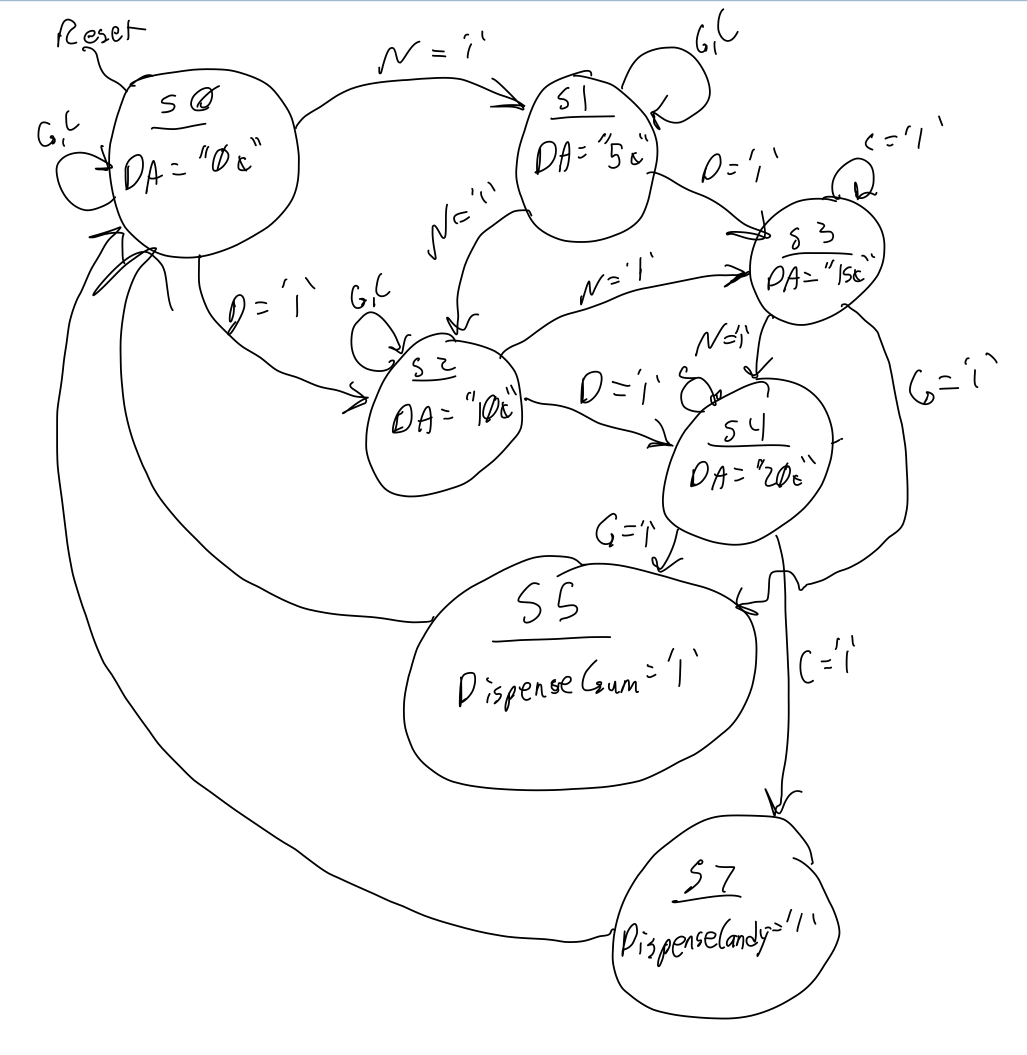
\includegraphics[width=\textwidth]{./img10_1.png}
	\caption{\label{fig:state_machine}State machine for vending machine.}
\end{center}
\end{figure}

\section{Conclusion}
Finite state machines are very useful for designing fault-tolerant systems that cycle through a set number of states based on limited inputs from users. We are now able to understand and design such systems. Being able to reduce state machines to the minimum number of states reduces hardware requirements and creates faster, more efficient systems.

\end{document}